\documentclass[11pt]{article}
\usepackage[margin=1in]{geometry}
\usepackage{graphicx}
\usepackage{hyperref}
\usepackage{amsmath}
\usepackage{booktabs}
\usepackage{caption}
\usepackage{subcaption}

% Use Roman numerals for sections and capital letters for subsections
\renewcommand{\thesection}{\Roman{section}}
\renewcommand{\thesubsection}{\Alph{subsection}}

\title{IBM Project 3 --- Implementing Paged Attention in FMS Using Flex Attention}
\author{
  Thomas Joshi (ttj2108) \and
  Neil Dhillon (nsd2147) \and
  Herman Saini (hss2173)
}
\date{\today}

\begin{document}

\maketitle
\begin{abstract}
% TODO: Summarize the goal of integrating Paged Attention into IBM's Foundation Model Stack (FMS) using Flex Attention, highlight expected memory and speed benefits, and mention benchmarks to be run.
\end{abstract}

\tableofcontents
\newpage

\section{Introduction}
  \subsection{Background and Motivation}
  % TODO: High‑level context on large‑context LLMs, attention bottlenecks, and FMS.
  
  \subsection{Problem Statement}
  % TODO: Explain limitations of current KV‑cache strategies and fused kernels.
  
  \subsection{Objectives and Scope}
  % TODO: Bullet the project goals listed in the proposal.

\section{Literature Review}
  \subsection{Review of Relevant Literature}
  \subsubsection{Paged Attention and vLLM}
  % TODO: Summarize Paged Attention and prior art (e.g.\ vLLM paper).

  \subsubsection{Flex Attention and FlashAttention}
  % TODO: Discuss Flex Attention library and related fused‑kernel work.

  \subsubsection{Memory‑Efficient Attention Strategies}
  % TODO: Briefly cover other approaches (Longformer, MQA/GQA, etc.).

  \subsection{Identification of Gaps in Existing Research}
  % TODO: Summarize open questions unaddressed by prior work.

\section{Methodology}
  \subsection{Data Collection and Preprocessing}
  % TODO: List H100/A100 specs, CUDA, PyTorch 2.1, FMS version.

  \subsection{Model Selection}
  \subsubsection{Custom KV‑Page Allocator}
  % TODO
  \subsubsection{Index Mapping \& Mask Modulation}
  % TODO
  \subsubsection{Kernel Fusion with \texttt{torch.compile}}
  % TODO

  \subsection{Optimization Procedures}
  % TODO: Synthetic vs real‑world long‑context corpora.

  \subsection{Profiling Tools and Methods}
  % TODO: Throughput (tokens/s), latency, GPU‑mem, accuracy.

  \subsection{Evaluation Metrics}
  % TODO: Define throughput, latency, memory footprint, and accuracy metrics.

\section{Experimental Results}
  \subsection{Experimental Setup}
  % TODO: Describe testbed configuration and run parameters.

  \subsection{Performance Comparison (before and after optimizations) of Different Models}
  \subsubsection{Throughput and Latency}
  % TODO: Insert tables/figures.
  \subsubsection{Memory Utilization}
  % TODO
  \begin{figure}[h]
    \centering
    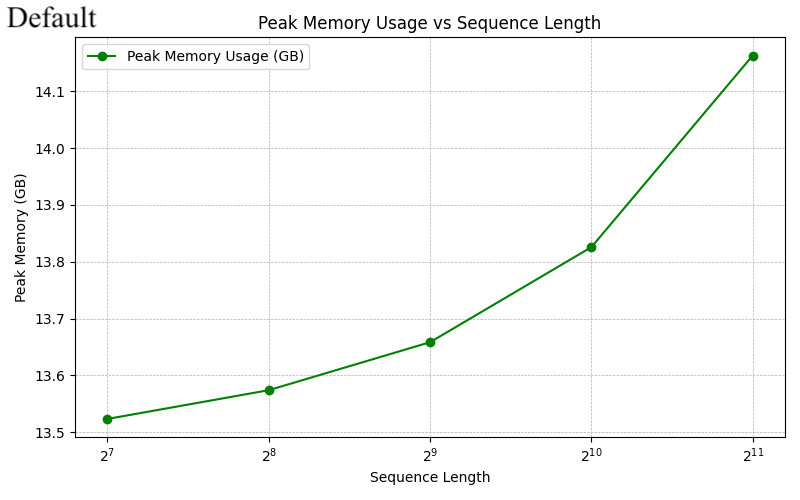
\includegraphics[width=0.7\textwidth]{../profile_memory_default_plot.png}
    \caption{Peak Memory Usage vs Sequence Length (Default Attention)}
  \end{figure}
  \begin{figure}[h]
    \centering
    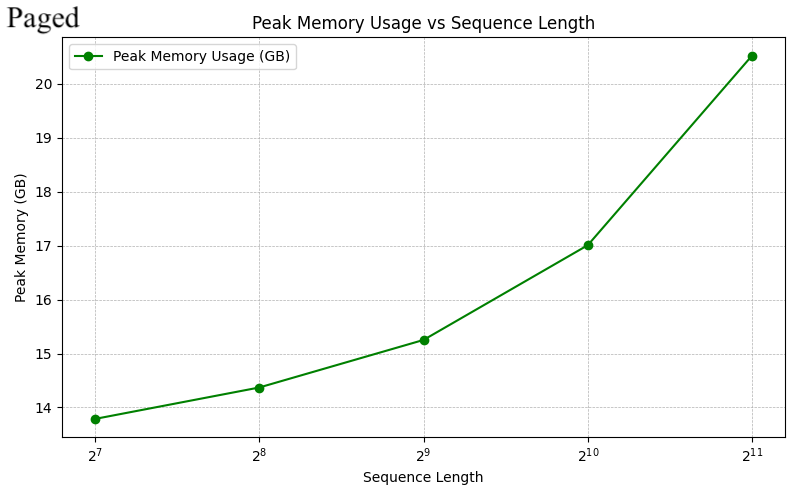
\includegraphics[width=0.7\textwidth]{../profile_memory_paged_plot.png}
    \caption{Peak Memory Usage vs Sequence Length (Paged Attention)}
  \end{figure}
  \subsubsection{Accuracy Impact}
  % TODO

  \subsection{Ablation Studies}
  % TODO: Page size sensitivity, paging heuristic variants, etc.

  \subsection{Analysis of Results}
  % TODO: Provide consolidated insight into experimental findings.

\section{Discussion}
  \subsection{Interpretation of Results}
  % TODO
  \subsection{Comparison with Previous Studies}
  % TODO
  \subsection{Challenges and Limitations}
  % TODO
  \subsection{Future Work}
  % TODO

\section{Conclusion}
\subsection{Summary of Findings}
% TODO

\subsection{Contributions}
% TODO

\subsection{Recommendations for Future Research}
% TODO

\section{References}
\bibliographystyle{plain}
\bibliography{references}

\appendix
\section{Project Proposal}
% Optional: Include the full proposal text.

\section{Additional Figures}
% TODO: Place extra plots as needed.

\end{document}